\documentclass[11pt]{article}

\usepackage[margin=1in]{geometry}
\usepackage{graphicx}

\graphicspath{{./images/}}

\title{Chapter 2 Exercises}
\author{Kyler Krenzke}
\date{}

\begin{document}

	\maketitle

	\begin{enumerate}
		\item \textbf{Exercise 2.1: In $\epsilon$-greedy action selection, for the case of two actions and $\epsilon=0.5$, what is the probability that the greedy action is
		selected?}

		0.75
		
		\item \textbf{Exercise 2.2 (Bandit example): Consider a k-armed bandit problem with $k=4$ actions, denoted 1, 2, 3, and 4. Consider applying to this problem a bandit
		algorithm using $\epsilon$-greedy action selection, sample-average action-value estimates, and initial estimates of $Q1(a)=0$, for all $a$. Suppose the initial sequence of
		actions and rewards is $A_1=1$, $R_1=-1$, $A_2=2$, $R_2=1$, $A_3=2$, $R_3=-2$, $A_4=2$, $R_4=2$, $A_5=3$, $R_5=0$. On some of these time steps the e case may have occurred,
		causing an action to be selected at random. On which time steps did this definitely occur? On which time steps could this possibly have occurred?}

		The epsilon case definitely occurred for $A_4=2$ because $A_2=2$ and $A_3=2$ received an average reward of -1 which would be less than the other initally zero valued
		states. It should also be noted, however, that any or all of these five actions could be epsilon cases and they randomly selected the greedy option.
		
		\item \textbf{Exercise 2.3: In the comparison shown in Figure 2.2, which method will perform best in the long run in terms of cumulative reward and probability of
		selecting the best action? How much better will it be? Express your answer quantitatively.}
		
		The method utilizing epsilon greedy search with an epsilon value of 0.01 will perform best in the long run in terms of cumulative reward and probability of selecting the
		best action because it will converge to a probability of $1-e$ of selecting the optimal action. Given that, it is trivial that $1-0.01 > 1-0.1$.
		
		\item \textbf{Exercise 2.4: If the step-size parameters, $\alpha_n$, are not constant, then the estimate $Q_n$ is a weighted average of previously received rewards with a
		weighting different from that given by (2.6). What is the weighting on each prior reward for the general case, analogous to (2.6), in terms of the sequence of step-size
		parameters?}
		
		$$\prod_{i=1}^N(1-\alpha_i)Q_1 + \sum_{i=1}^N(\alpha_i * \prod_{j=i+1}^N (1 - \alpha_j) * R_i)$$
		
		\item \textbf{Exercise 2.5 (programming): Design and conduct an experiment to demonstrate the difficulties that sample-average methods have for nonstationary problems. Use
		a modified version of the 10-armed testbed in which all the $q(a)$ start out equal and then take independent random walks (say by adding a normally distributed increment
		with mean 0 and standard deviation 0.01 to all the $q(a)$ on each step). Prepare plots like Figure 2.2 for an action-value method using sample averages, incrementally
		computed, and another action-value method using a constant step-size parameter, $\alpha=0.1$. Use $\epsilon=0.1$ and longer runs, say of 10,000 steps.}
		
		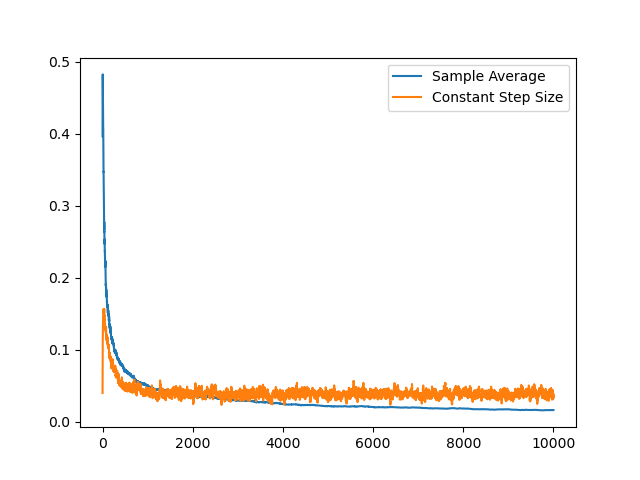
\includegraphics[scale=.5]{average_rewards}
		
		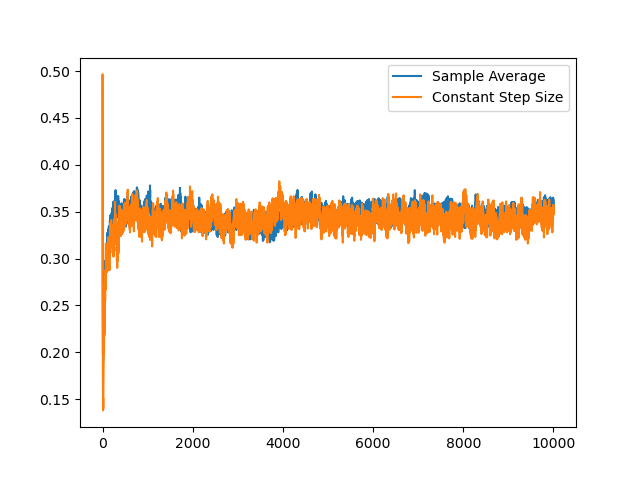
\includegraphics[scale=.5]{optimal_action}
		
		Code in exercise25.py
		
		\item \textbf{Exercise 2.6 (Mysterious Spikes): The results shown in Figure 2.3 should be quite reliable because they are averages over 2000 individual, randomly chosen
		10-armed bandit tasks. Why, then, are there oscillations and spikes in the early part of the curve for the optimistic method? In other words, what might make this method
		perform particularly better or worse, on average, on particular early steps?}
		
		The early oscillations and spikes could be caused by the initial optimism of the agent. In the case that the initial action values are not selected optimistically, the
		action values start at zero and slowly decrease their bias towards the true values. In the case of optimistic initial values, however, the first few trials for each action
		will have a much larger effect on the estimated action values causing them to decrease quickly. This lets the agent explore more freely in the early trials. Since it
		explore more freely earlier, it also has a higher percentage likelihood to select the optimal action at an earlier time. Once it starts to converge, the optimistic action
		percentage drops way down and the rate of increase becomes more typical.
		
		\item \textbf{Exercise 2.7 (Unbiased Constant-Step-Size Trick): In most of this chapter we have used sample averages to estimate action values because sample averages do
		not produce the initial bias that constant step sizes do (see the analysis leading to (2.6)). However, sample averages are not a completely satisfactory solution because
		they may perform poorly on nonstationary problems. Is it possible to avoid the bias of constant step sizes while retaining their advantages on nonstationary problems? One
		way is to use a step size of $\beta_n=\alpha_n/\bar{o}_n$, to process the $n$th reward for a particular action, where $\alpha>0$ is a conventional constant step size, and
		$\bar{o}_n$ is a trace of one that starts at 0: $\bar{o}_n=\bar{o}_{n-1}+\alpha(1-\bar{o}_{n-1})$ for $n\geq0$, with $\bar{o}_0=0$. Carry out an analysis like that in
		(2.6) to show that $Q_n$ is an exponential recency-weighted average \textit{without initial bias}.}
		
		$Q_n$ is an exponential recency-weighted average without initial bias if the step size $\alpha$ obeys the following two rules: (1) $\sum_{n=1}^\infty\alpha_n(a)=\infty$
		and (2) $\sum_{n=1}^\infty \alpha^2_n(a)<\infty$.
		
		$Q_n$ is an exponential recency-weighted average using the step-size of $\beta_n$,
		
		$$Q_{n+1}=Q_n+\beta_n[R_n-Q_n]$$
		$$=\beta_nR_n+(1-\beta_n)Q_n$$
		$$=\beta_nR_n+(1-\beta_n)[\beta_{n-1}+(1-\beta_{n-1}Q_{n-1}]$$
		$$=\prod_{i=1}^N(1-\beta_1)Q_1 + \sum_{i=1}^N(\beta_i * \prod_{j=i+1}^N(1-\beta_j)R_j)$$
		
		$Q_n$ does not have initial bias,
		
		$$\sum_{n=1}^\infty\beta_n(a)=\sum_{n=1}^\infty\alpha/\bar{o}_n=\alpha\sum_{n=1}^\infty1/\bar{o}=\infty$$
		$$\sum_{n=1}^\infty\beta^2_n(a)=\sum_{n=1}^\infty\alpha^2/\bar{o}^2_n=\alpha^2 \sum_{n=1}^\infty 1/\bar{o}^2<\infty$$
		
		\item \textbf{Exercise 2.8 (UCB Spikes): In Figure 2.4 the UCB algorithm shows a distinct spike in performance on the 11th step. Why is this? Note that for your answer to
		be fully satisfactory it must explain both why the reward increases on the 11th step and why it decreases on the subsequent steps. Hint: if c = 1, then the spike is less
		prominent.}
		
		
		
	\end{enumerate}
	
\end{document}